\documentclass[a4paper]{article}
\usepackage{graphicx}
\usepackage{xcolor}
\usepackage{url}
\usepackage{outlines}
\usepackage{listings}
\usepackage{fontspec}
\lstset{basicstyle=\ttfamily,
	showstringspaces=false,
	commentstyle=\color{blue},
	keywordstyle=\color{pink}
}
\lstset{emph={
	EXPOSE,RUN,FROM,CMD,nc,tcp,udp,http,docker},emphstyle=\color{purple}
}
\newcommand{\abc}{\hfill \break}
\newcommand{\ii}{\textit}
\usepackage{fancyhdr}
\usepackage{geometry}
% \usepackage{hyperref}
% \hypersetup{
% 	colorlink=true,
% 	linktoc=all,
% 	linkcolor=pink,
% }
\geometry{
	a4paper,
	total={170mm,257mm},
	left=20mm,
	top=20mm,
	bottom=39mm,
}

\setlength{\headheight}{82.70538pt}

\fancypagestyle{oida}{
	\fancyhf{}
	\fancyhead[L]{\fontsize{7.5}{7.5}htl donaustadt\\ Donaustadtstraße 45\\
		1220 Wien\\~\\ Abteilung: Informationstechnologie\\ 
	Schwerpunkt: Netzwerktechnik}
	\fancyhead[R]{
\includegraphics[scale=0.45]{images/logo.png}}

	\fancyfoot[L]{\today}
	\fancyfoot[C]{\jobname}
	\fancyfoot[R]{Seite: \thepage}
}

\begin{document}
\pagestyle{oida}
\section*{Configure Basic Router Settings}
\par\noindent\rule{\textwidth}{0.4pt}

Laboratory protocol
Configure Basic Router Settings

\begin{figure}[h]
	
\includegraphics[scale=0.2]{images/mika.jpeg}
	\centering
\end{figure}

\vspace*{\fill}
Subject:	NWT|ANGE

Class:	3AHITN

Name:	Stefan Fürst, Marcel Raichle

Group Name/Number: Dumm und Dümmer/7

Supervisor: 	ANGE

Exercise dates:	

Submission date:


\newpage
\tableofcontents

\newpage

\section{Task definition}



\section{Summary}


\newpage

\section{Exercise Execution}
\subsection{Set Up the Topology and Initialize Devices}
This exercise was done in Cisco Packet Tracer and the devices were placed and wired using the automatic cabling type, as all the devices are Auto-MDIX compliant anyway.\abc
\begin{figure}[h]
	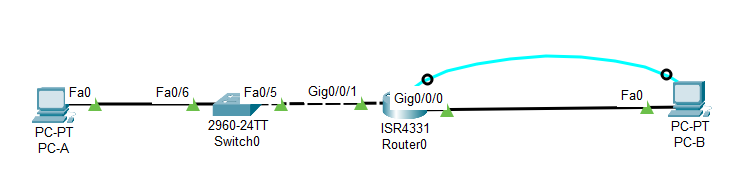
\includegraphics[scale=0.45]{images/nwtopology.png}
	\centering
	\caption{Network topology required for this exercise}
\end{figure}\abc
After that, everything was turned on and the router and switch were both iniliazised and reloaded.

\subsection{Configure Devices and Verify Connectivity}
\subsubsection{Configure the PC interfaces}
The IP addresses for both PCs have been set in the IP Configuration application.
\begin{figure}[h]
	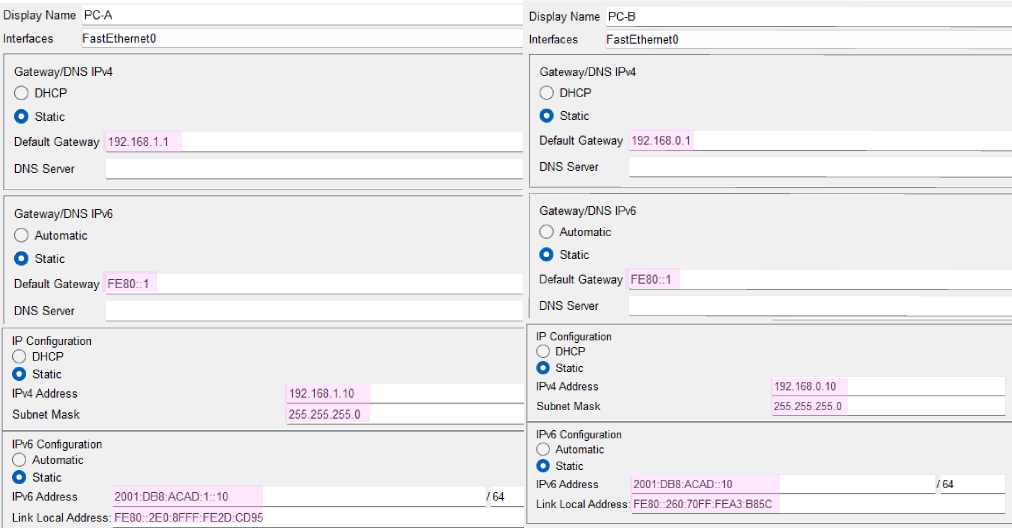
\includegraphics[scale=0.45]{images/pc-ipconf.png}
	\centering
	\caption{IP configuration for PC-A and PC-B}
\end{figure}
\newpage
\subsection{Configure the router}
To access the router's configuration mode, connect to the router through the console port and execute the \ii{en} and \ii{conf t} commands.\abc
The following basic settings are configured using the commands listed below:
\begin{lstlisting}[language=bash]
#setting the hostname
hostname R1
#setting the domain name of the router
ip domain name ccna-lab.com
#disable DNS lookup on mistyped commands
no ip domain lookup
#encrypting plaintext passwords
service password-encryption
security passwords min-length 12
\end{lstlisting}

\newpage
\section{List of figures}

\listoffigures

\end{document}
